\documentclass[a4paper,12pt]{article} 

%%% Работа с русским языком
\usepackage{cmap}                           % поиск в PDF
\usepackage{mathtext} 			 	       % русские буквы в формулах
\usepackage[T2A]{fontenc}               % кодировка
\usepackage[utf8]{inputenc}              % кодировка исходного текста
\usepackage[english,russian]{babel}  % локализация и переносы
\usepackage{wrapfig}
\usepackage{gensymb}
\usepackage{textcomp}
\usepackage{multirow}
\usepackage{amsmath,amsfonts,amssymb,amsthm,mathtools} % AMS
\usepackage{euscript}	 % Шрифт Евклид
\usepackage{mathrsfs} % Красивый матшрифт
\usepackage{graphicx}%Вставка картинок правильная
\usepackage{float}%"Плавающие" картинки
\usepackage{wrapfig}%Обтекание фигур (таблиц, картинок и прочего)
\title{Лабораторная работа 2.5.1 

Измерение коэффициента поверхностного натяжения жидкости}
\author{Кагарманов Радмир Б01-106}
\date{11 апреля 2022 г.}
\begin{document}

\maketitle
\newpage
\paragraph{Цель работы:}1) измерение температурной зависимости  коэффициента поверхностного натяжения дистиллированной воды с использованием известного коэффициента поверхностного натяжения спирта;  2) определение полной поверхностной энергии  и теплоты, необходимой для изотермического образования единицы  поверхности жидкости  при различной температуре.
\paragraph{В работе используется:}прибор  Ребиндера  с термостатом и микроманометром; исследуемые жидкости; стаканы.
\paragraph{Теория\\}
Наличие поверхностного слоя приводит к различию давлений по разные стороны от искривленной границы раздела двух сред.  Для сферического пузырька с воздухом  внутри жидкости избыточное давление даётся формулой Лапласа:
\begin{equation}
    \Delta P = P_{\text{вн}} - P_{\text{сн}} = \dfrac{2 \sigma}{r}
\end{equation}
где $\sigma$ - коэффициент поверхностного натяжения, $P_{\text{вн}}$ и $P_{\text{сн}}$ - давление внутри пузырька и снаружи, $r$ - радиус кривизны поверхности раздела двух фаз. Эта формула лежит в основе предлагаемого метода определения коэффициента поверхностного натяжения жидкости. Измеряется давление $\Delta P$, необходимое для выталкивания в жидкость пузырька воздуха.
\paragraph{Экспериментальная установка\\}
Исследуемая жидкость (дистиллированная вода) наливается в сосуд (колбу) В (рис.1). Тестовая жидкость  (этиловый спирт) наливается  в сосуд Е.  При измерениях  колбы герметично закрываются  пробками.   Через одну из двух пробок  проходит полая металлическая игла С. Этой пробкой закрывается сосуд, в котором  проводятся измерения. Верхний конец иглы открыт в атмосферу, а нижний погружен в жидкость. Другой сосуд герметично закрывается второй пробкой. При создании достаточного  разряжения воздуха в колбе с иглой пузырьки воздуха начинают пробулькивать через жидкость. Поверхностное натяжение можно определить по величине разряжения $\Delta P$ (1), необходимого для прохождения пузырьков (при известном радиусе иглы).\\
Разряжение в системе создается с помощью аспиратора А. Кран $\text{K}_2$ разделяет две полости аспиратора. Верхняя полость при закрытом кране $\text{K}_2$  заполняется водой. Затем кран $\text{K}_2$ открывают и заполняют водой  нижнюю полость  аспиратора.  Разряжение воздуха создается в нижней полости  при открывании крана $\text{K}_1$, когда  вода вытекает из неё по каплям. В колбах В и С, соединённых трубками с нижней полостью аспиратора,  создается такое же пониженное давление. Разность давлений в полостях с разряженным воздухом и атмосферой измеряется спиртовым микроманометром. \\
Для стабилизации температуры исследуемой жидкости через рубашку D колбы В непрерывно прогоняется вода из термостата.
\begin{figure}[h]
    \centering
    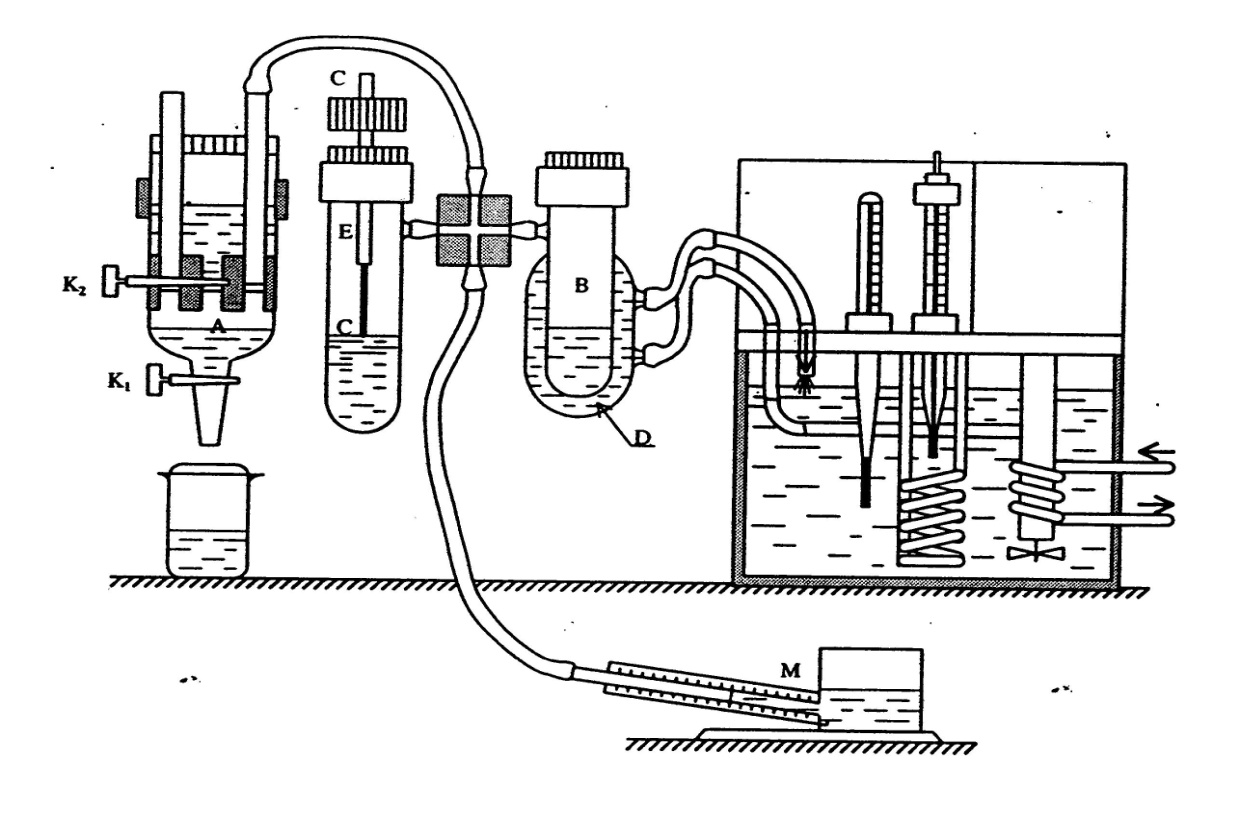
\includegraphics[width=0.5\linewidth]{Установка.jpg}
    \caption{Экспериментальная установка}
    \label{fig:my_label}
\end{figure}
\paragraph{Ход работы и обработка результатов}
\subparagraph{1.}Измеряем $d$ иглы по формуле (1) и с помощью микроскопа. $\Delta P = (147\pm 2) \text{Па}$.
\begin{center}
    $d_{\text{ф}}=(1,23\pm 0,02)\text{мм}$\\
    $d_{\text{м}}=(1,20\pm 0,05)\text{мм}$
\end{center}
\subparagraph{2.}Помещаем иглу в пробирку с водой. При комнатной температуре измеряем $h_1$ и $h_2$ относительно неподвижной детали. Найдём $\rho g\Delta h$. $P_1=(223,7\pm 2,0)\text{Па},~P_2=(408,1\pm 2,0)\text{Па}$. По формуле найдём $\Delta h_{\text{ф}}=\frac{P_2-P_1}{\rho g}$
\begin{center}
    $\Delta h_{\text{л}}=(1,70\pm 0,01)см$\\
    $\Delta h_{\text{ф}}=(1,84\pm 0,04)см$\\
    $\rho g \Delta h = (184,4 \pm 4,0)Па$
\end{center}
$\sigma$ для комнатной температуры равна $(0,06711\pm 0,00301)~Н/м$.
\subparagraph{3.}Снимем температурную зависимость $\sigma(T)$ для воды. В таблице 1 измерения этой зависимости. 
\newpage
\begin{table}[h]
    \centering
    \begin{tabular}{|c|c|c|c|c|c|c|c|c|c|}
    \hline
        $t,~ \degree C$ & \multicolumn{7}{|c|}{$P,~Па$} & $P_{\text{ср}}, ~ Па$ & $\sigma,~ Н/м$ \\ \hline
        25,5 & 412,0 & 402,2 & 400,2 & 400,2 & 392,4 & 396,3 & 396,3 & 400,0 & 0,0647 \\ \hline
        30,4 & 412,0 & 412,0 & 410,1 & 410,1 & 408,1 & 406,1 & 406,1 & 410,1 & 0,0677 \\ \hline
        35,3 & 412,0 & 410,1 & 408,1 & 408,1 & 406,1 & 408,1 & 406,1 & 408,4 & 0,0672 \\ \hline
        40,1 & 412,0 & 410,1 & 408,1 & 406,1 & 408,1 & 408,1 & 408,1 & 408,7 & 0,0673 \\ \hline
        45,2 & 404,2 & 404,2 & 402,2 & 404,2 & 402,2 & 402,2 & 402,2 & 403,3 & 0,0657 \\ \hline
        50,1 & 398,3 & 396,3 & 398,3 & 400,2 & 400,2 & 400,2 & 400,2 & 399,1 & 0,0644 \\ \hline
        55,0 & 392,4 & 394,4 & 394,4 & 396,3 & 396,3 & 396,3 & 398,3 & 395,5 & 0,0633 \\ \hline
        59,0 & 390,4 & 390,4 & 388,5 & 392,4 & 392,4 & 392,4 & 392,4 & 391,3 & 0,0621 \\ \hline
    \end{tabular}
    \caption{Caption}
    \label{tab:my_label}
\end{table}
Во время измерения $\Delta h$ я снял дополнительную рубашку с пробирки с водой и забыл надеть обратно, поэтому некоторые измерения с зависимостью $\sigma (T)$ были без неё. Начиная с температуры 40,1 я надел её, и коэффициент поверхностного начал стабильно падать. Первые температуры не будут включены в график.
\begin{figure}[h]
    \centering
    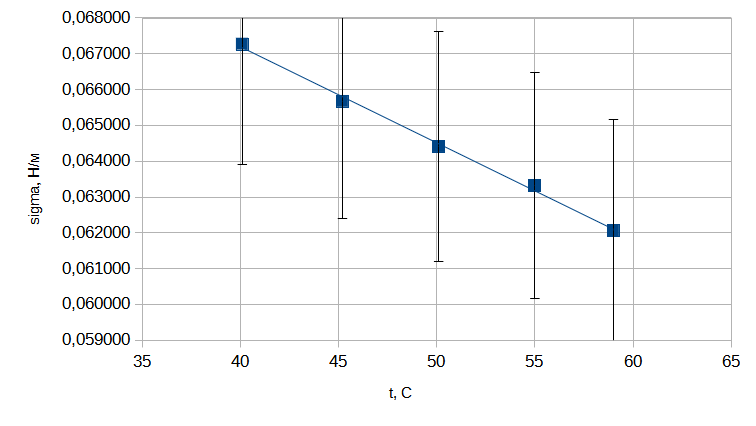
\includegraphics[width=0.7\linewidth]{sigmaT.png}
    \caption{График зависимости $\sigma(t)$}
    \label{fig:my_label}
\end{figure}\\
При применении МНК получаем $\frac{d\sigma}{dT}=0,000269~\frac{Н}{м\cdot \degree C}$. С учётом погрешности $\sigma$ и МНК: $\frac{d\sigma}{dT}=(0,000269\pm 0,000021)~\frac{Н}{м\cdot \degree C}$.
\subparagraph{4.}На рисунке 3 представлены зависимости теплоты образования единицы поверхности жидкости $q$ и поверхностной энергии $U$ единицы площади $F$.
\begin{figure}[h]
    \centering
    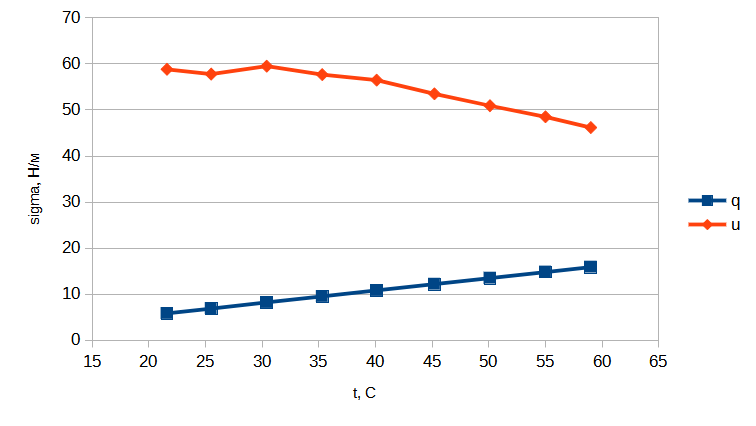
\includegraphics[width=0.7\linewidth]{gr.png}
    \caption{График зависимости $\sigma(t)$}
    \label{fig:my_label}
\end{figure}\\
\newpage
\paragraph{Вывод:}проделав данную лабораторную работу, был найден коэффициент поверхностного натяжения воды при комнатной температуре $\sigma = (0,06711\pm 0,00301)~Н/м$. Результат похож  на табличное значение, но не совпадает с ним. Также мы сняли зависимость $\sigma$ от $T$, и $\frac{d\sigma}{dT}$ получилось $(0,000269\pm 0,000021)~\frac{Н}{м\cdot \degree C}$.
\end{document}
